\documentclass[BTech]{nitkdiss}
%\documentclass[12pt, a4paper]{report}

\usepackage{amsmath,amssymb,graphicx,color,colortbl}
\usepackage{hyperref}


\title{Real-time 3D sound realization}

\author{Bilal Ali(15EC112)\\Sathwik G S (15EC116)\\ Barun Kumar Acharya (15EC209)\\}
\mentor{Dr. Sumam David}
\date{\today}
\department{Electronics and Communication Engineering}

\begin{document}
\maketitle
\pagestyle{plain}
\pagenumbering{arabic}

\newpage
\begin{abstract}
3D Audio is a generic name that encompasses ways to render audio like in reality and in particular its spatial dimension; it is the capability to produce and perceive sounds in any direction and at any distance. Localization of sounds in physical space plays a very important role in multiple audio-related disciplines.

  Binaural recording is the most commonly used method to provide an immersive sound experience by means of headphone reproduction.The method is based on a time-frequency analysis of the spatial properties of the sound picked up by a simple dual microphone array, assuming source sparseness. 
  Usually  ,  in  order  to synthesize 3D  sound effects  using  binaural  
systems,  we  use  Head-related    transfer    functions    (HRTFs)    to  describe    the    spectral  
filtering    that  occurs  between    a    source  sound  and  the  listener’s  eardrum.  Because  of  the  
characteristics  of  HRTF  some  three-dimensional  effects  in  the  area  of  a  cone  of  confusion  
between front and back directions can be declined. In order to design the system , we derive a large 
set  of  HRTFs  for  different  azimuth  and  elevations  from already present databases and with the help other binaural cues reconstruct the signal to generate the appropriate effect. 
In  this  project  we implement a system for 3D  sound  localization which synthesizes a signal in real-time and aim to achieve with minimal computational complexity. The output sound  quality  is  
evaluated by a subjective listening test. 
\end{abstract}
\tableofcontents

\chapter{Introduction}
\section{ Problem definition } 
We are trying to design a system that will enable the user to realize and virtually locate a sound source heard through headphones. However, the main criteria of this system would be to respond in real-time.
This has become a hot topic in the past few years due to its expanding application in a lot of fields like games, home theaters and human aid systems.  It can improve our experience in some interactive application together with haptic feedback.  
\section{Previous work}
The first and foremost is the amplitude panning method used
in stereo and surround systems today which was invented in 1931 by Alan Blumlein. This method is designed to allow audio sources to be placed at different angular offsets whichs allows instruments to be placed in different positions to build up a sound scene utilising the sine/cosine panning law (Tomlinson, 2000), or in more advanced cases in surround systems to place sources around a listener in the horizontal plane.

HRTF’s (head related transfer functions) allow
localisation of sources in the vertical dimension.It was proposed by Wallach (1939) that dynamic head movements also facilitate the localisation of sources in the vertical dimension due to head movements which produce variations in inter-aural differences to resolve the position of sources in the vertical dimension.
Recent research by Ashby et al. (2011) investigated the influence of head rotation on the localisation of elevated sound sources. They used a multi microphone sphere consisting of four pairs of omni-directional microphones distributed around the equator of a plastic sphere.


\section{Motivation}
People hear sound in three dimensions and the perception of the spatial aspects of sound has been essential to human survival.Psycho-acoustic researchers have been studying this problem from the view of understanding the functioning of the human hearing system which makes sound
localization possible in the real world, leading to the principles of binaural human hearing. Binaural means that hearing or listening uses only two ears. 

A well known example is stereo reproduction, which can provide a sense of
directionality because sounds can be heard from different directions within the angle subtended by the loudspeakers by simply manipulating the gains assigned to the source in each channel (i.e., amplitude panning ). The result is that stereo reproduction, though pleasant, falls far short of reproducing realistic listening environment. 


\section{Overview}          
The setup includes a dual microphone arrangement which continuously records and the recorded sound is further filtered. This filtered sound is then played back over headphones. The selection of the filter is based on the location of the sound source w.r.t the center of the microphone setup. Filters are parametrized based on the azimuth and angle of elevation value . \newline
In order to calculate the angle of sound source, we cross-correlate the signals observed on both the microphones and calculate the delay between them. Once this is calculated, appropriate filter is chosen and convolved with the recorded signals. Typically, sounds generated from headphones appear to originate from within the head. In the virtual auditory space, the headphones should be able to “externalize” the sound. Using the HRTF, sounds can be spatially positioned.

\chapter{Background and Implementation}
\section{How do we hear 3D sound with only two ears?}
The auditory system uses the combination of 2 types of information to localize a sound: \textbf{Binaural Cues} (Time and Level) and \textbf{Head Related Transfer Functions} (HRTF).
\subsection{Binaural Cues}
When a sound source is located eccentrically, it is closer to one ear than the other and sound arrives later and weaker at one ear. Time and level difference perception between the two ears provide information about direction. These binaural cues are called Inter-aural Time Difference (ITD) and Inter-aural Level Difference (ILD). They are important for the horizontal localisation. The auditory system evaluates interaural time differences from: (a) Phase delays at low frequencies and (b) group delays at high frequencies. Interaural Intensity Difference (IID) or Interaural Level Difference (ILD) are highly frequency dependent and they increase with increasing frequency. Massive theoretical researches demonstrate that IID relates to the signal frequency f and the angular position of the acoustic source θ. The function of IID is given by:
 \begin{equation}
IID = 1.0 + \frac{f}{1000}^{0.8} \times sin\theta
\end{equation}
\begin{figure}[h!]
  \centering
  \begin{minipage}[b]{0.3\textwidth}
    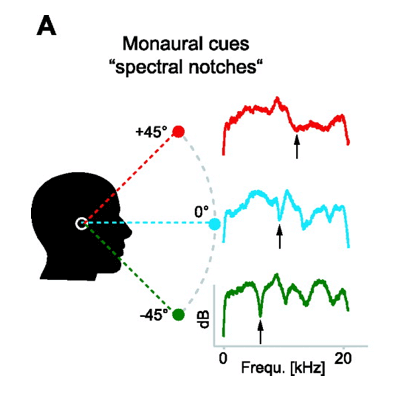
\includegraphics[width=\textwidth]{A}
  \end{minipage}
  \hfill
  \begin{minipage}[b]{0.3\textwidth}
    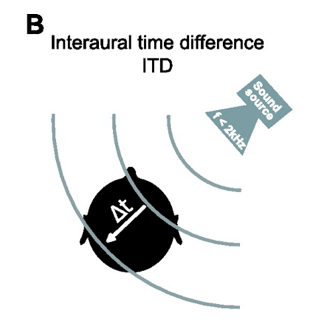
\includegraphics[width=\textwidth]{B}
  \end{minipage}
  \begin{minipage}[b]{0.3\textwidth}
    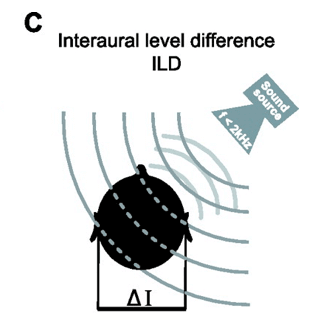
\includegraphics[width=\textwidth]{C}
  \end{minipage}
\end{figure}
For frequencies below 1000 Hz, mainly ITDs are evaluated (phase delays), for frequencies above 1500 Hz mainly IIDs are evaluated. Between 1000 Hz and 1500 Hz there is a transition zone, where both mechanisms play a role.
\subsection{HRTF}
Before reaching the entrance of the ear canal, a sound wave coming from one direction is transformed by the multiple reflections on our body, our face and more importantly our ears. This transformation, called Head Related Transfer Function (HRTF), is different for each direction of sound and has a specific spectral signature for each direction. It is a transfer function, describing how a sound from a specific point will arrive at the ear (generally at the outer end of the auditory canal). The brain has “learned” these signature over time and when it hears a sound with a specific signature, it can find out its direction in its HRTF memory. HRTF is important for vertical localization. A pair of HRTFs for two ears can be used to synthesize a binaural sound that seems to come from a particular point in space. 
\begin{figure}[!tbp]
  \centering
  \begin{minipage}[b]{0.45\textwidth}
    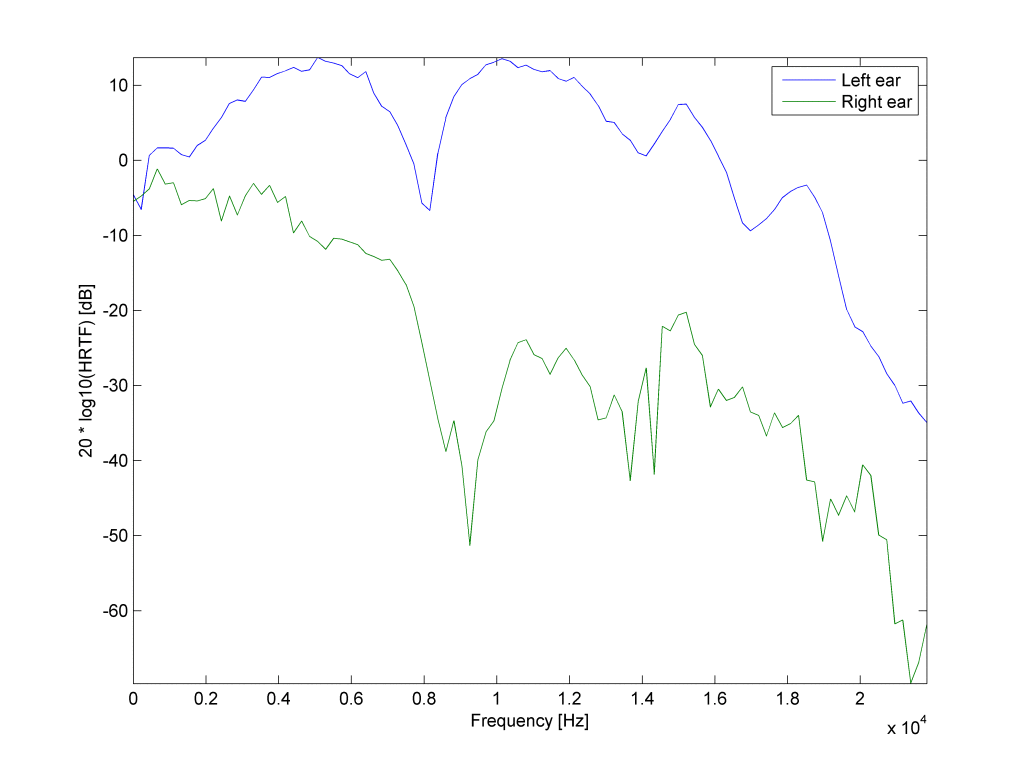
\includegraphics[width=\textwidth]{hrtf_left}
    \caption{HRTF for source to the left}
  \end{minipage}
  \hfill
  \begin{minipage}[b]{0.45\textwidth}
    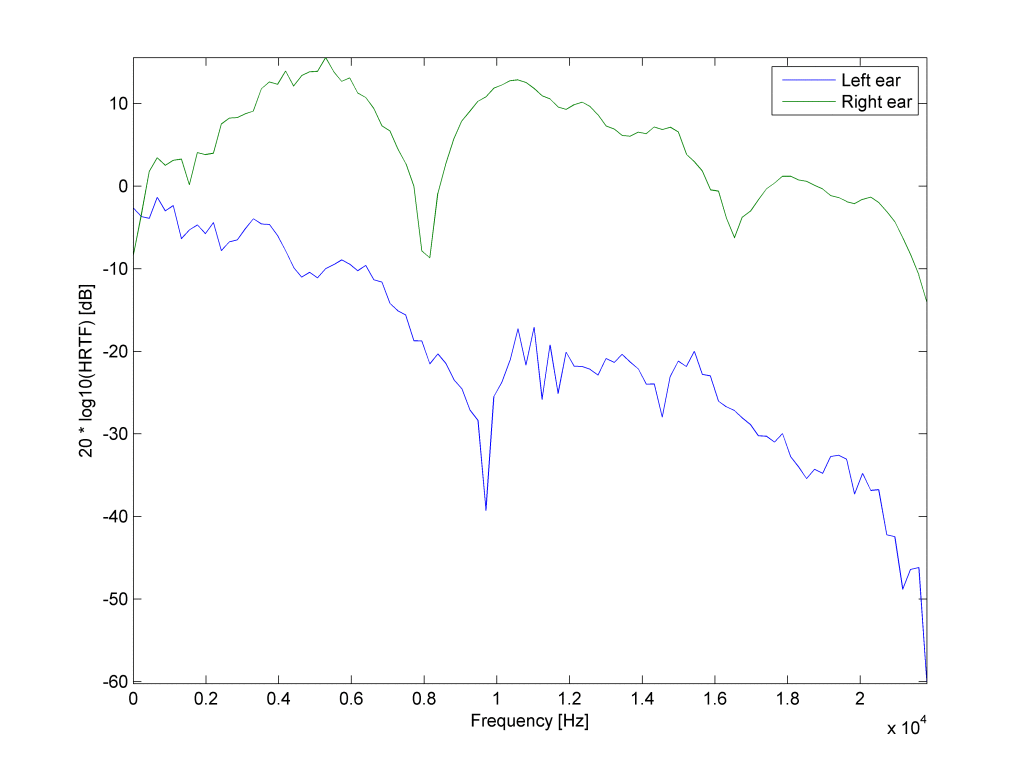
\includegraphics[width=\textwidth]{hrtf_right}
    \caption{HRTF for source to the right }
  \end{minipage}
\end{figure}
HRTFs are typically measured in an anechoic chamber to minimize the influence of early reflections and reverberation on the measured response. HRTFs are measured at small increments of θ such as 15$^{\circ}$ or 30$^{\circ}$ in the horizontal plane, with interpolation used to synthesize HRTFs for arbitrary positions of θ. Even with small increments, however, interpolation can lead to front-back confusion, and optimizing the interpolation procedure is an active area of research. 
\section{HRTF Database}
The area of 3D sound synthesis has been active since a very long time and many research labs have collected the HRIR (Head related impulse response) in well structured environment suitable for audio recordings. Some of these databases are from MIT, UC Davis (CIPIC database) and few privately funded labs. \newline
The database is maintained based on recordings from different subjects (with varying anthropometric data). Each subject is equipped with a pair of microphones and is made to sit in an anechoic chamber. Test sounds are played and the perceived signals on each ear is recorded. These sounds are played from different azimuthal as well as elevated angles. Some of the database includes anthropometric measurements for use in HRTF scaling studies.
\begin{figure}
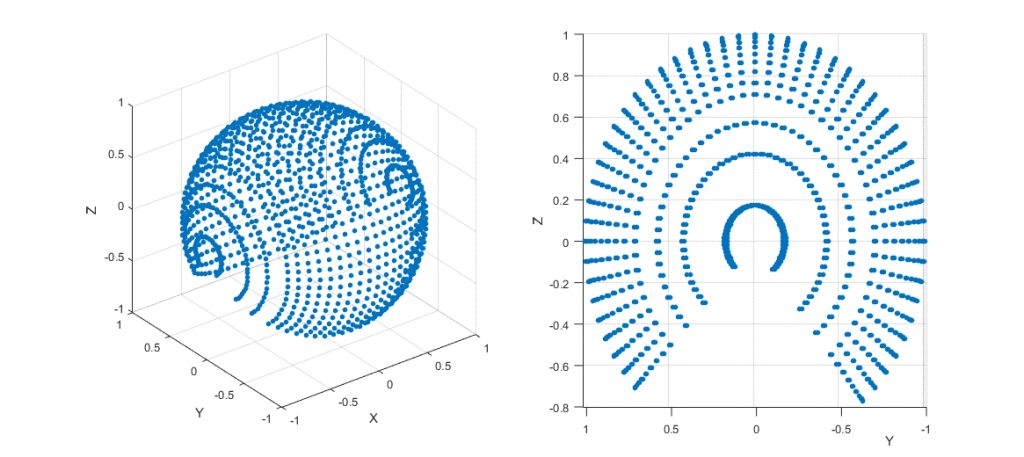
\includegraphics[width = \textwidth]{data_points}
\caption{Visualization of points at which HRIR from CIPIC are recorded.}
\end{figure}
\section{The setup}
%Record with 2 microphones
The system we plan to design receives audio input , gets filtered and is played back through headphones with 3D-like effect. \newline
For collecting audio samples, we recorded audio input using 2 microphones separated by 20cm (approximate distance between two ears). We used the National Instruments Data Acquisition module to simultaneously record the input from 2 microphones at 48 kHz sampling rate. The recorded data were passed as text files to MATLAB environment for further processing .
%correlation & angle resolution
\subsection{MATLAB}
The hrtf database was loaded along with the audio file. Cross-correlation between input received at left microphone and the input received at the right microphone was performed. Based upon the results of cross-correlation , we get the time difference of arrival of audio input at the left microphone and the right microphone. Based on this time difference, we can predict the azimuthal and spatial information of the audio source. 
\begin{equation}
\tau = \frac{Max(S_{L} * S_{R}) - Signal length}{Sampling Frequency} 
\end{equation}
where '*' operator denotes the cross-correlation operation on left and right microphone signals. 

\begin{equation}
Sin\theta = \frac{\tau c}{d}
\end{equation}
where c is speed of sound in air , d is 20cm, $\theta$ is azimuthal angle .

%Software
Based on the above values, a particular HRTF filter was chosen and convolved with the input. The output we observed showed features clearly indicating spatial properties. In the same way we tested for different azimuthal angles using its corresponding HRTF filter coefficients.
\chapter{Observations and analysis}
Here are some of the observations, which were observed while experimenting with different audio samples and different HRTF filters.  
\section{Observation}
\subsection{Angle resolution}
When the signals were correlated to get the difference in time of arrival for both microphones, for source angle range of 0$^{\circ}$ - 90$^{\circ}$ the number of distinct values (for Sampling rate = 48 kHz) was 28.
\begin{equation}
0^\circ - 90^\circ = 28 (values)
\end{equation}
Therefore, each increment in value of $\tau$ index results in change in angle of 3.2$^\circ$.
\subsection{Panning}
Panning is the spread of a monaural signal in a stereo or multi-channel sound field. Here, we realize different directions of sound source by changing the filters accordingly. The resultant effect when heard will be equivalent to as if the source is moving around the head. 
\begin{figure}[h!]
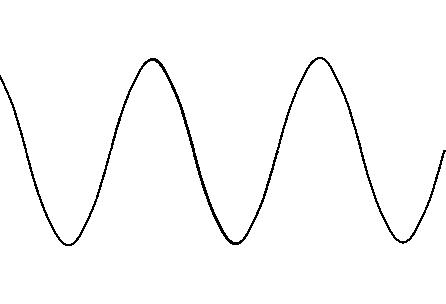
\includegraphics[width = \textwidth, height = 5cm]{sine}
\caption{Input: Sine wave of 1kHz}
\end{figure}
\begin{figure}[h!]
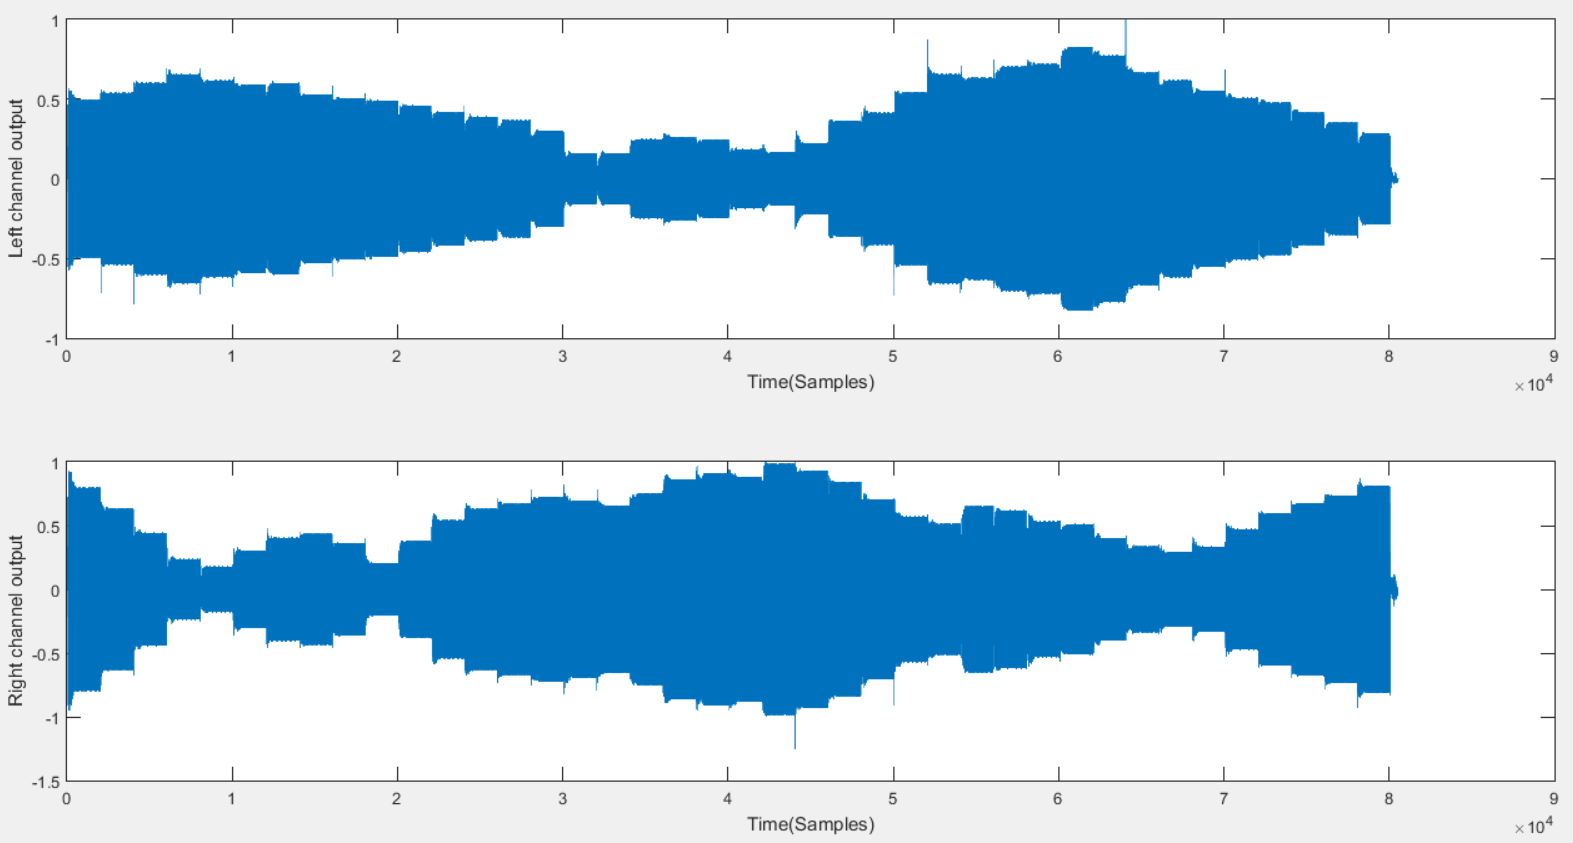
\includegraphics[width = \textwidth, height = 8cm]{output_sine}
\caption{Output: After panning}
\end{figure}
We can clearly see that whenever the filter applied is changed , the output changes abruptly giving rise to effects like audio glitches/cracks. Though this effect is not quite audible but exists.  

\section{Further work to be done}
\begin{itemize}
\item Hardware design of the complete system (Using cadence)
\item Optimization in storing and processing of filters
\item Interpolation of filter coefficients 
\item Include Gyroscope + accelerometer sensor to track head movement in real-time and accordingly filter

\end{itemize}

\begin{bibliography}{9}

\end{bibliography}

\end{document}
